\section{Charge transport and the measured charge}\label{sec:20.1}

The charge amplifier of a semiconductor detector integrates the current that flows into an electrode while the carriers move, and a carrier that is captured halfway across the crystal leaves half a charge in the integral and does half its share of Luke work. As a result, the charge we read is the pair number $N_{\mathrm{eh}}$ of \cref{sec:18.2} times a gain that depends on where the event happened and how far each carrier got, and the fluctuations of that gain add to the fluctuations of the cascade. At millikelvin temperatures the carriers drift in fields of a few V/cm, trapped charge does not escape thermally, and every drifting carrier radiates phonons. We will see that trapping lowers the read charge and the Luke heat by the same factor, but spreads the read charge in a way that no pair statistics removes.

\subsection{Induced charge and Ramo's theorem}\label{sec:20.1-ramo}

Consider electrodes $k$ held at potentials $V_k$ around a crystal with static dielectric constant $\varepsilon_0$ (a pure number in the Heaviside--Lorentz units of the book, \cref{sec:5.5}), and a point charge $q$ inside at $\vect{r}$. The charge on electrode $s$ is the sum of what the bias puts there and what $q$ induces, and in a linear medium the two add. The induced part follows from Green's reciprocity theorem. Compare two configurations of the same conductors. In the first, $q$ is at $\vect{r}$ and every electrode is grounded, and electrode $k$ carries the induced charge $Q_k^{\mathrm{ind}}$. In the second, there is no charge inside, electrode $s$ is held at unit potential and the others are grounded; the potential inside is then the \emph{weighting potential} $\varphi_s(\vect{r})$, the solution of $\nabla\cdot[\varepsilon_0(\vect{r})\nabla\varphi_s] = 0$ with $\varphi_s = 1$ on electrode $s$ and 0 on the others. Reciprocity states that the sum of the charges of one configuration times the corresponding potentials of the other is the same either way round. The first configuration has charges $Q_k^{\mathrm{ind}}$ on the electrodes and $q$ at $\vect{r}$; in the second the electrode potentials are $\delta_{ks}$ and the potential at $\vect{r}$ is $\varphi_s(\vect{r})$. The second configuration has charges only on the electrodes, and in the first all the electrodes are grounded. Hence $Q_s^{\mathrm{ind}} + q\varphi_s(\vect{r}) = 0$. When $q$ moves from $\vect{r}_1$ to $\vect{r}_2$, the external circuit must supply the change in induced charge, and the charge delivered to electrode $s$ is
\begin{equation}
  \Delta Q_s = -q\,\bigl[\varphi_s(\vect{r}_2) - \varphi_s(\vect{r}_1)\bigr] ,
  \label{eq:20.1-ramo}
\end{equation}
with the current $I_s = -q\,\vect{v}\cdot\nabla\varphi_s$ in its lead while the carrier moves at velocity $\vect{v}$. This is the Shockley--Ramo theorem~\cite{shockley1938currents,ramo1939currents}, \cite[Eq.~(2)]{lachish2017electron}. The weighting potential is a property of the electrode geometry alone. It is not the potential the carrier moves in. The applied bias, other carriers and trapped charges change the field and the trajectory, but by linearity they only add their own contributions to $Q_s$, and the charge induced by $q$ at a given point stays the same. \Cref{eq:20.1-ramo} is therefore exact in the presence of space charge.

For two planar electrodes at $z = 0$ and $z = d_{\mathrm{det}}$, the weighting potential of the electrode at $z = d_{\mathrm{det}}$ is $\varphi = z/d_{\mathrm{det}}$. Let the electrode at $z = d_{\mathrm{det}}$ collect electrons (the anode), so that holes drift toward the cathode at $z = 0$. Let a pair be born at depth $z$, and let its electron drift a path $s_e$ toward the anode and its hole a path $s_h$ toward the cathode. By \cref{eq:20.1-ramo} the pair delivers the charge $e\,\mathfrak{q}$ to the anode, with
\begin{equation}
  \mathfrak{q} = \frac{s_e + s_h}{d_{\mathrm{det}}} , \qquad 0 \le s_e \le d_{\mathrm{det}} - z, \quad 0 \le s_h \le z .
  \label{eq:20.1-qpair}
\end{equation}
A pair that is fully collected gives $\mathfrak{q} = 1$ wherever it was born, since its two carriers together cross the whole thickness $d_{\mathrm{det}}$. A pair born at the midplane gives $\frac12 + \frac16 = \frac23$ if its hole arrives at the cathode and its electron is captured a third of the way to the anode.

The same theorem gives the work of the bias. To hold electrode $k$ at $V_k$ while the charge it carries changes by $\Delta Q_k$, its source does the work $V_k\Delta Q_k$. Summing \cref{eq:20.1-ramo} over the electrodes gives the work done on a carrier that moves from $\vect{r}_1$ to $\vect{r}_2$, $-q\sum_kV_k[\varphi_k(\vect{r}_2) - \varphi_k(\vect{r}_1)]$. The sum $\varphi_{\mathrm{bias}}(\vect{r}) \equiv \sum_kV_k\varphi_k(\vect{r})$ is the potential the electrodes produce in the empty crystal, so that
\begin{equation}
  W_{\mathrm{bias}} = \sum_{\text{carriers}} q\,\bigl[\varphi_{\mathrm{bias}}(\vect{r}_{\mathrm{start}}) - \varphi_{\mathrm{bias}}(\vect{r}_{\mathrm{end}})\bigr] .
  \label{eq:20.1-work}
\end{equation}
The bias work is the carrier charge times the drop of $\varphi_{\mathrm{bias}}$ along the path, whatever space charge is present. Between two planes at $0$ and $V_{\mathrm{bias}}$, $\varphi_{\mathrm{bias}} = V_{\mathrm{bias}}z/d_{\mathrm{det}}$, and each pair contributes $eV_{\mathrm{bias}}\mathfrak{q}$: this is \cref{eq:19.5-Wbias}, $W_{\mathrm{bias}} = eV_{\mathrm{bias}}N_{\mathrm{ind}}$, with $N_{\mathrm{ind}} = \sum_i\mathfrak{q}_i$ the charge read on the anode in units of $e$. \Cref{app:D.45} shows that the Luke heat is $W_{\mathrm{bias}}$ minus the change $\Delta E_{\mathrm{es}}$ of the electrostatic energy. For a single trapped pair that change is negligible. Two charges \SI{10}{\micro m} apart in silicon have the Coulomb energy $\alpha/(\varepsilon_0r) = \SI{1.3e-5}{eV}$, with the liquid-helium value $\varepsilon_0 = 11.4$ (\cref{sec:7.4}), against the bias work $eV_{\mathrm{bias}}s/d_{\mathrm{det}} = \SI{4}{meV}$ done on a carrier over those \SI{10}{\micro m} in a \SI{1}{cm} crystal at \SI{4}{V}.

With more than two electrodes the read charge and the bias work weight a trajectory differently. The charge read on electrode $s$ follows $\varphi_s$ and the work follows $\varphi_{\mathrm{bias}}$, and the read charge and the bias work are proportional only where $\varphi_s \propto \varphi_{\mathrm{bias}}$, as for a pair of planar electrodes. Some detectors place interleaved electrodes on each face to tag events close to a surface. Near the interleaved electrodes the weighting potentials change over the electrode pitch, and a carrier that is trapped there adds to the read charge and to the bias work in proportions that differ from its share of the path. The reconstruction $E_R = E_\phi - E_QeV_{\mathrm{bias}}/\varepsilon_{\mathrm{eh}}$ of \cref{sec:19.5} subtracts the Luke heat through the read charge $E_Q$, and for carriers trapped near the faces it inherits the mismatch between the read charge and the bias work.

\subsection{Trapping and the Hecht relation}\label{sec:20.1-hecht}

A drifting carrier at millikelvin temperatures is lost when an ionized or neutral impurity captures it, with the cross-sections $\sigma_{\mathrm{cap},j}$ of \cref{sec:18.5}. If capture events are independent, the probability of surviving a further path $\dd s$ is $1 - \dd s/\lambda_{\mathrm{d}}$, and the probability of surviving a path $s$ is $\ee^{-s/\lambda_{\mathrm{d}}}$. The drift length is $\lambda_{\mathrm{d}} = 1/\sum_j\nd^{\mathrm{tr}}_j\sigma_{\mathrm{cap},j}$ for trap densities $\nd^{\mathrm{tr}}_j$ and cross-sections taken per unit path; with a trapping time $\tau_{\mathrm{tr}}$ instead, $\lambda_{\mathrm{d}} = v_{\mathrm{dr}}\tau_{\mathrm{tr}}$ with the drift velocity $v_{\mathrm{dr}}$. Electrons and holes have separate drift lengths, $\lambda_{\mathrm{d}}^e$ and $\lambda_{\mathrm{d}}^h$. For a path that is exponentially distributed but cut off at the distance $L$ to the electrode, the mean is $\langle\min(s, L)\rangle = \lambda_{\mathrm{d}}(1 - \ee^{-L/\lambda_{\mathrm{d}}})$.

The classic measurement of the drift length creates the charge at one face, with an alpha source or a short-range photon, so that one carrier type crosses the whole crystal and the other is collected at once. By \cref{eq:20.1-qpair} the mean collected fraction is then the mean path over $d_{\mathrm{det}}$,
\begin{equation}
  \frac{Q}{eN_{\mathrm{eh}}} = \frac{\lambda_{\mathrm{d}}}{d_{\mathrm{det}}}\bigl(1 - \ee^{-d_{\mathrm{det}}/\lambda_{\mathrm{d}}}\bigr) ,
  \label{eq:20.1-hecht}
\end{equation}
the Hecht relation~\cite{hecht1932mechanismus}, \cite[Eqs.~(1)--(4)]{lachish2017electron}. It is linear in $\lambda_{\mathrm{d}}$ for $\lambda_{\mathrm{d}} \ll d_{\mathrm{det}}$, where the carriers stop after a mean path $\lambda_{\mathrm{d}}$, and approaches $1 - d_{\mathrm{det}}/2\lambda_{\mathrm{d}}$ for $\lambda_{\mathrm{d}} \gg d_{\mathrm{det}}$. Dark-matter events happen anywhere in the bulk, and both carriers then drift. With the cut-off mean path for each carrier, a pair at depth $z$ induces on average
\begin{equation}
  \bar{\mathfrak{q}}(z) = \frac{\lambda_{\mathrm{d}}^e}{d_{\mathrm{det}}}\Bigl(1 - \ee^{-(d_{\mathrm{det}} - z)/\lambda_{\mathrm{d}}^e}\Bigr) + \frac{\lambda_{\mathrm{d}}^h}{d_{\mathrm{det}}}\Bigl(1 - \ee^{-z/\lambda_{\mathrm{d}}^h}\Bigr) ,
  \label{eq:20.1-hecht2}
\end{equation}
and averaging over a uniform depth,
\begin{equation}
  \langle\bar{\mathfrak{q}}\rangle = \sum_{c = e, h}\frac{\lambda_{\mathrm{d}}^c}{d_{\mathrm{det}}}\Bigl[1 - \frac{\lambda_{\mathrm{d}}^c}{d_{\mathrm{det}}}\bigl(1 - \ee^{-d_{\mathrm{det}}/\lambda_{\mathrm{d}}^c}\bigr)\Bigr] \simeq 1 - \frac{d_{\mathrm{det}}}{6\lambda_{\mathrm{d}}^e} - \frac{d_{\mathrm{det}}}{6\lambda_{\mathrm{d}}^h} .
  \label{eq:20.1-qavg}
\end{equation}
At second order in $d_{\mathrm{det}}/\lambda_{\mathrm{d}}$ each carrier adds $+d_{\mathrm{det}}^2/24\lambda_{\mathrm{d}}^2$, so the leading correction is accurate to a fraction $d_{\mathrm{det}}/4\lambda_{\mathrm{d}}$ of itself. Each carrier of a bulk event loses a third of what the carrier of a face event loses at the same drift length: for $\lambda_{\mathrm{d}} \gg d_{\mathrm{det}}$ the loss over a path $L$ is $L^2/2\lambda_{\mathrm{d}}d_{\mathrm{det}}$, and the mean square path to an electrode is $d_{\mathrm{det}}^2/3$. \Cref{fig:20-hecht} compares a face event, a uniform bulk event and an event at the midplane. At $\lambda_{\mathrm{d}} = d_{\mathrm{det}}$ the face event collects 0.632 of its charge, the uniform bulk event 0.736 and the midplane event 0.787; at $\lambda_{\mathrm{d}} = 10\,d_{\mathrm{det}}$ the face and bulk values are 0.952 and 0.968. The dependence of the induced charge on depth, \cref{fig:20-hecht}(b), turns trapping into a spread of the read charge (\cref{sec:20.1-fano}).

\begin{figure}[tbp]
  \centering
  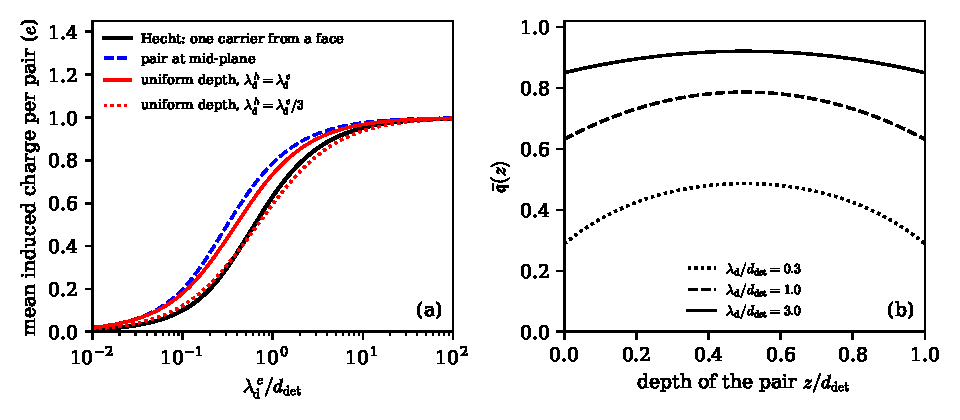
\includegraphics[width=\linewidth]{figures/ch20/fig20_1.pdf}
  \caption{Charge collection with exponential trapping in a planar detector of thickness $d_{\mathrm{det}}$. (a)~Mean induced charge per pair, in units of $e$, against the electron drift length: the Hecht relation \cref{eq:20.1-hecht} for one carrier crossing from a face (black), a pair at the midplane with equal drift lengths (blue dashed), and the depth average \cref{eq:20.1-qavg} for uniform events with $\lambda_{\mathrm{d}}^h = \lambda_{\mathrm{d}}^e$ (red) and $\lambda_{\mathrm{d}}^h = \lambda_{\mathrm{d}}^e/3$ (red dotted, an illustrative ratio). (b)~Mean induced charge of a pair against its depth, \cref{eq:20.1-hecht2} with equal drift lengths $0.3$, $1$ and $3\,d_{\mathrm{det}}$; the electron-collecting electrode is at $z = d_{\mathrm{det}}$.}
  \label{fig:20-hecht}
\end{figure}

Hecht wrote the drift length as $\lambda_{\mathrm{d}} = \mu_{\mathrm{mob}}\tau_{\mathrm{tr}}V_{\mathrm{bias}}/d_{\mathrm{det}}$, for a drift velocity proportional to the field, $v_{\mathrm{dr}} = \mu_{\mathrm{mob}}\mathcal{E}$ with mobility $\mu_{\mathrm{mob}}$, and a field-independent trapping time. The standard way to obtain the mobility--lifetime product is to measure $Q$ against the bias and fit \cref{eq:20.1-hecht} in this form. Neither the proportional drift velocity nor the field-independent trapping time enters the derivation above, which needs only exponential survival along the path. At millikelvin temperatures both assumptions fail. A carrier accelerates until it moves faster than sound and then sheds its energy into Luke phonons (\cref{sec:20.1-luke}); its speed stays within a few times the sound speed, and the largest momentum it reaches grows only as the cube root of the field~\cite[Eqs.~(24)--(25)]{leman2012invited}. If the capture cross-section per unit path does not depend on the carrier speed, $\lambda_{\mathrm{d}}$ is independent of the bias and the collected fraction does not change with the bias. If capture is a rate at fixed trapping time, $\lambda_{\mathrm{d}} = v_{\mathrm{dr}}\tau_{\mathrm{tr}}$ stops growing once the velocity saturates, and the collected fraction saturates below one.

\begin{limitbox}[Hecht collection][lim:20.1a]
For charge created at one face and drifting in a uniform field~\cite{hecht1932mechanismus}, \cite[Eqs.~(1)--(4)]{lachish2017electron}: $Q/eN_{\mathrm{eh}} = (\lambda_{\mathrm{d}}/d_{\mathrm{det}})(1 - \ee^{-d_{\mathrm{det}}/\lambda_{\mathrm{d}}})$ with $\lambda_{\mathrm{d}} = \mu_{\mathrm{mob}}\tau_{\mathrm{tr}}V_{\mathrm{bias}}/d_{\mathrm{det}}$.
\par\smallskip
{\centering
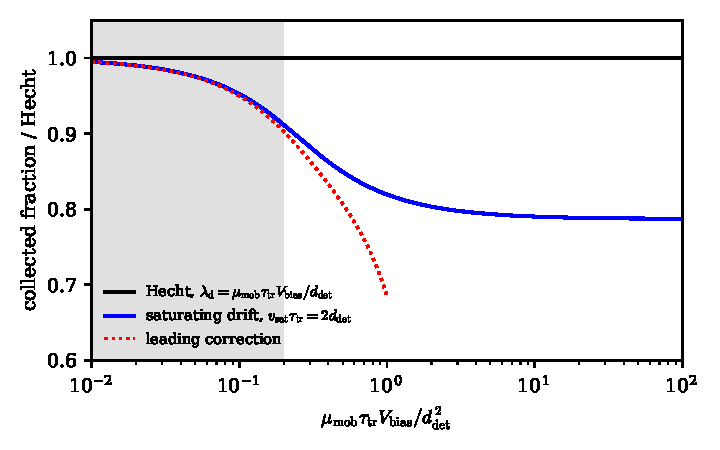
\includegraphics[width=\linewidth]{figures/ch20/limit20_1a.pdf}
\captionof{figure}{Collected fraction with a saturating drift velocity divided by the Hecht relation, against the bias in units of $d_{\mathrm{det}}^2/\mu_{\mathrm{mob}}\tau_{\mathrm{tr}}$. Blue: \cref{eq:20.1-hecht} with $\lambda_{\mathrm{d}} = v_{\mathrm{dr}}\tau_{\mathrm{tr}}$ and the interpolation $v_{\mathrm{dr}} = \mu_{\mathrm{mob}}\mathcal{E}/(1 + \mu_{\mathrm{mob}}\mathcal{E}/v_{\mathrm{sat}})$, at $v_{\mathrm{sat}}\tau_{\mathrm{tr}} = 2\,d_{\mathrm{det}}$ (an illustrative value). Red dotted: the leading correction, $\lambda_{\mathrm{d}} = \mu_{\mathrm{mob}}\tau_{\mathrm{tr}}\mathcal{E}(1 - \mu_{\mathrm{mob}}\mathcal{E}/v_{\mathrm{sat}})$. Gray: $\mu_{\mathrm{mob}}\mathcal{E} \le 0.1\,v_{\mathrm{sat}}$, where the deficit relative to the Hecht relation is at most \SI{8.9}{\percent}. At high bias the collected fraction saturates at 0.787 of the charge instead of approaching one.}\label{fig:20-limit-hecht}
\par}
\smallskip
Once the drift velocity no longer follows the field, the collected charge stops rising with the bias, and a fit of the Hecht form returns a mobility--lifetime product that depends on the bias range used.
\end{limitbox}

The deficit of the collected fraction relative to the Hecht relation is $\mu_{\mathrm{mob}}\mathcal{E}/v_{\mathrm{sat}}$ to first order, since the collection is linear in $\lambda_{\mathrm{d}}$ while $\lambda_{\mathrm{d}} \ll d_{\mathrm{det}}$. If the survival law is not exponential, as when the trap occupation changes during the drift, \cref{eq:20.1-hecht} itself changes.

\subsection{Bias work with trapping}\label{sec:20.1-work}

Trapping lowers the Luke heat with the read charge. On average over a uniform depth, \cref{eq:20.1-work} gives $W_{\mathrm{bias}} = eV_{\mathrm{bias}}N_{\mathrm{eh}}\langle\bar{\mathfrak{q}}\rangle$, and for an electron recoil that deposits $\omega$ the Luke phonon energy is $g_{\mathrm{Luke}}\langle\bar{\mathfrak{q}}\rangle\,\omega$, with the Luke gain $g_{\mathrm{Luke}} = eV_{\mathrm{bias}}/\varepsilon_{\mathrm{eh}}$ of \cref{sec:19.5}. The published phonon energy (\cref{lim:20.1b}) counts every pair as fully collected.

\begin{limitbox}[Bias work and the Luke phonon energy][lim:20.1b]
The phonon energy of $n_Q$ pairs drifted across the bias $V_{\mathrm{bias}}$ is $E_\phi = E_R + n_QeV_{\mathrm{bias}}$, with Luke part $n_QeV_{\mathrm{bias}}$~\cite[Eq.~(1)]{agnese2018nuclear}.
\par\smallskip
{\centering
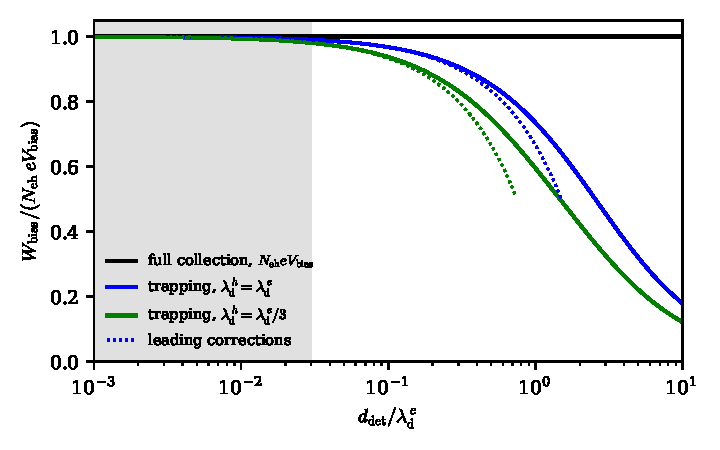
\includegraphics[width=\linewidth]{figures/ch20/limit20_1b.pdf}
\captionof{figure}{Bias work of uniformly distributed events with exponential trapping, \cref{eq:20.1-work} with the depth average \cref{eq:20.1-qavg}, over the full-collection value $N_{\mathrm{eh}}eV_{\mathrm{bias}}$, against the crystal thickness in units of the electron drift length. Blue: equal drift lengths; green: $\lambda_{\mathrm{d}}^h = \lambda_{\mathrm{d}}^e/3$ (an illustrative ratio). Dotted: the leading correction $1 - d_{\mathrm{det}}/6\lambda_{\mathrm{d}}^e - d_{\mathrm{det}}/6\lambda_{\mathrm{d}}^h$. Gray: $d_{\mathrm{det}} \le 0.030\,\lambda_{\mathrm{d}}$, where the work is within \SI{1}{\percent} of full collection for equal drift lengths ($d_{\mathrm{det}} \le 0.015\,\lambda_{\mathrm{d}}^e$ for the unequal pair).}\label{fig:20-limit-work}
\par}
\smallskip
When the drift length is no longer much longer than the crystal, the Luke heat falls below $N_{\mathrm{eh}}eV_{\mathrm{bias}}$ and depends on the depth of the event; it follows the read charge, not the pair number.
\end{limitbox}

Since the read charge of a planar detector carries the same factor $\bar{\mathfrak{q}}$ as the Luke heat, event by event, the subtraction $E_QeV_{\mathrm{bias}}/\varepsilon_{\mathrm{eh}}$ removes the Luke heat of partly collected pairs exactly. Trapping also changes the signal beyond the Luke heat. A trapped carrier keeps its share of the gap energy, which the balance law counts as missing energy (\cref{sec:19.5}), and a nuclear recoil has an ionized fraction $f_{\mathrm{ion}}$ below its ionization yield if its dense track traps more often.

\subsection{Fano factor of the measured charge}\label{sec:20.1-fano}

If each pair is either collected in full or lost, independently and with the same probability $f_{\mathrm{det}}$ everywhere, the read charge is the pair number thinned binomially, and its Fano factor is $f_{\mathrm{det}}F_{\mathrm{eh}} + 1 - f_{\mathrm{det}}$ by \cref{eq:C.11-thinfano}. Trapping does not thin the pair number binomially. A trapped carrier leaves a partial charge, and the mean collection depends on the depth of the event. Let the event be at $\vect{r}$, and let the induced charges $\mathfrak{q}_i$ of its pairs, \cref{eq:20.1-qpair}, be independent and identically distributed given $\vect{r}$, with mean $\bar{\mathfrak{q}}(\vect{r})$ and variance $\sigma_{\mathfrak{q}}^2(\vect{r})$, and independent of the pair number. These assumptions hold when the carriers drift independently after the prompt cascade; independent drift excludes recombination and screening inside a dense track. The read charge is $N_{\mathrm{ind}} = \sum_{i=1}^{N_{\mathrm{eh}}}\mathfrak{q}_i$. At fixed $\vect{r}$, a sum of a random number of independent terms has mean $\bar N_{\mathrm{eh}}\bar{\mathfrak{q}}$ and variance $\bar N_{\mathrm{eh}}\sigma_{\mathfrak{q}}^2 + \bar{\mathfrak{q}}^2\operatorname{Var}N_{\mathrm{eh}}$, with $\operatorname{Var}N_{\mathrm{eh}} = F_{\mathrm{eh}}\bar N_{\mathrm{eh}}$. Averaging over the position with the law of total variance gives $\operatorname{Var}N_{\mathrm{ind}} = \langle\operatorname{Var}(N_{\mathrm{ind}}|\vect{r})\rangle + \operatorname{Var}_{\vect{r}}(\bar N_{\mathrm{eh}}\bar{\mathfrak{q}})$, and dividing by the mean $\bar N_{\mathrm{eh}}\langle\bar{\mathfrak{q}}\rangle$ gives
\begin{equation}
  F_{\mathrm{meas}} = \underbrace{\frac{F_{\mathrm{eh}}\langle\bar{\mathfrak{q}}^2\rangle}{\langle\bar{\mathfrak{q}}\rangle}}_{\text{cascade}} + \underbrace{\frac{\langle\sigma_{\mathfrak{q}}^2\rangle}{\langle\bar{\mathfrak{q}}\rangle}}_{\text{partial charge}} + \underbrace{\bar N_{\mathrm{eh}}\,\frac{\operatorname{Var}_{\vect{r}}\bar{\mathfrak{q}}}{\langle\bar{\mathfrak{q}}\rangle}}_{\text{position}} ,
  \label{eq:20.1-Fpos}
\end{equation}
where $\langle\cdot\rangle$ and $\operatorname{Var}_{\vect{r}}$ are taken over the distribution of event positions.

For all-or-nothing collection with one probability, $\bar{\mathfrak{q}} = f_{\mathrm{det}}$, $\sigma_{\mathfrak{q}}^2 = f_{\mathrm{det}}(1 - f_{\mathrm{det}})$ and the position term vanishes; \cref{eq:20.1-Fpos} then returns the binomial result. The unsplit excitons of \cref{eq:18.5-Fmeas} are the same thinning with $f_{\mathrm{det}} = 1 - p_{\mathrm{ns}}$, and the values of $f_{\mathrm{det}}$ of losses that act independently on each pair multiply. The partial-charge term is never larger than in the binomial case. Since $0 \le \mathfrak{q} \le 1$, $\mathfrak{q}^2 \le \mathfrak{q}$, so $\langle\mathfrak{q}^2\rangle \le \bar{\mathfrak{q}}$ and $\sigma_{\mathfrak{q}}^2 \le \bar{\mathfrak{q}}(1 - \bar{\mathfrak{q}})$ at every position. At a fixed position, a loss shared as partial charges by many pairs fluctuates less than the same mean loss concentrated on a few pairs that are lost entirely. The position term grows with $\bar N_{\mathrm{eh}}$, and its contribution to the relative variance of the read charge, $\operatorname{Var}_{\vect{r}}\bar{\mathfrak{q}}/\langle\bar{\mathfrak{q}}\rangle^2$, does not fall with energy. The position term is a spread of the gain across the crystal, which no pair statistics removes, and it dominates at large deposits.

\begin{workedexample}{The measured Fano factor at 95 percent collection in silicon}\label{we:20-fano}
Take the cascade value $F_{\mathrm{eh}} = 0.114$ of \cref{sec:18.2} and a mean collected fraction of 0.95, and compare three ways of losing the missing \SI{5}{\percent}. (\Cref{sec:20.5} uses the measured value 0.119 for electron-recoil signals.)

\emph{All-or-nothing loss, uniform.} Binomial thinning gives $0.95 \times 0.114 + 0.05 = 0.158$.

\emph{Trapping, every pair at the midplane.} With equal drift lengths, \cref{eq:20.1-hecht2} at $z = d_{\mathrm{det}}/2$ is $2(\lambda_{\mathrm{d}}/d_{\mathrm{det}})(1 - \ee^{-d_{\mathrm{det}}/2\lambda_{\mathrm{d}}})$, which equals 0.95 at $\lambda_{\mathrm{d}} = 4.83\,d_{\mathrm{det}}$. Each carrier's path is exponential with mean $\lambda_{\mathrm{d}}$, cut at $d_{\mathrm{det}}/2$, and its second moment is $\langle\min(s, L)^2\rangle = 2\lambda_{\mathrm{d}}^2[1 - \ee^{-L/\lambda_{\mathrm{d}}}(1 + L/\lambda_{\mathrm{d}})]$. The two carriers give $\sigma_{\mathfrak{q}}^2 = 0.0156$, a third of the binomial $0.95 \times 0.05 = 0.0475$. \Cref{eq:20.1-Fpos} gives $F_{\mathrm{meas}} = (0.114 \times 0.9025 + 0.0156)/0.95 = 0.125$.

\emph{Trapping, uniform depth.} Now \cref{eq:20.1-qavg} equals 0.95 at $\lambda_{\mathrm{d}} = 6.41\,d_{\mathrm{det}}$. Integrating \cref{eq:20.1-hecht2} and the variance over depth gives $\langle\bar{\mathfrak{q}}^2\rangle = 0.9026$, $\langle\sigma_{\mathfrak{q}}^2\rangle = 0.0230$ and $\operatorname{Var}_z\bar{\mathfrak{q}} = 1.16\times10^{-4}$. The cascade and partial-charge terms give 0.1325. The position term is $1.22\times10^{-4}\,\bar N_{\mathrm{eh}}$: 0.003 for a \SI{100}{eV} recoil ($\bar N_{\mathrm{eh}} = 26.7$), 0.033 at \SI{1}{keV} and 0.19 at \SI{5.9}{keV}. It equals 0.01 at 82 pairs, about \SI{0.3}{keV}.

The same mean collection thus yields a measured Fano factor between 0.125 and 0.158 at \SI{100}{eV}, depending on how the charge is lost, and nearly three times the cascade value at \SI{5.9}{keV} if the loss depends on depth. A Fano factor measured at \SI{5.9}{keV} constrains $F_{\mathrm{eh}}$ to 0.01 only if $\operatorname{Var}_z\bar{\mathfrak{q}}$ is below $6\times10^{-6}$.
\end{workedexample}

\subsection{Space charge of trapped carriers}\label{sec:20.1-space}

At millikelvin temperatures a trapped carrier is not re-emitted thermally. A donor level \SI{45}{meV} below the conduction band carries the Boltzmann factor $\ee^{-1.04\times10^4}$ at \SI{50}{mK}. A field lowers the Coulomb barrier of a charged center: the potential energy $-\alpha/(\varepsilon_0r) - e\mathcal{E}r$ of the carrier along the field has its maximum at the field separation radius $r_{\mathcal{E}} = (\alpha/\varepsilon_0e\mathcal{E})^{1/2}$ of \cref{eq:18.5-rfield}, and the field thus lowers the barrier by the Poole--Frenkel amount $2e\mathcal{E}r_{\mathcal{E}}$. In silicon that is \SI{0.45}{meV} at \SI{4}{V/cm} and \SI{2.25}{meV} at \SI{100}{V/cm}, far below \SI{45}{meV}. Thermal and field-assisted emission are frozen, and trapped charge is released only by the phonons of later events, by drifting carriers that ionize the center on impact, or by infrared light. Detectors are therefore illuminated at intervals with infrared diodes, a practice called flashing~\cite[Sect.~2]{agnese2018nuclear}; the infrared light neutralizes the ionized trapping sites and keeps trapping low. Between flashes the trapped charge accumulates and changes the field.

In a planar detector at fixed bias the field change follows from Gauss's law and the constraint that the voltage across the crystal does not change. Let $\varrho_{\mathrm{tr}}(z)$ be the net trapped charge per unit volume, averaged over the transverse directions. The field change obeys $\dd\Delta\mathcal{E}/\dd z = \varrho_{\mathrm{tr}}/\varepsilon_0$, so $\Delta\mathcal{E}(z) = \Delta\mathcal{E}(0) + \varepsilon_0^{-1}\int_0^z\varrho_{\mathrm{tr}}\,\dd z'$, and fixed bias requires $\int_0^{d_{\mathrm{det}}}\Delta\mathcal{E}\,\dd z = 0$. Solving for $\Delta\mathcal{E}(0)$ and integrating by parts gives
\begin{equation}
  \Delta\mathcal{E}(z) = \frac{1}{\varepsilon_0}\left[\int_0^z\varrho_{\mathrm{tr}}(z')\,\dd z' - \frac{1}{d_{\mathrm{det}}}\int_0^{d_{\mathrm{det}}}(d_{\mathrm{det}} - z')\,\varrho_{\mathrm{tr}}(z')\,\dd z'\right] ,
  \label{eq:20.1-dE}
\end{equation}
in Heaviside--Lorentz units, with $\varepsilon_0$ the static dielectric constant; in SI units multiply $\varepsilon_0$ by the vacuum permittivity $\varepsilon_0^{\mathrm{SI}}$. A sheet of $\nd_{\mathrm{sh}}$ charges $e$ per unit area at depth $z_0$ makes the field jump by $e\nd_{\mathrm{sh}}/\varepsilon_0$ across it, with the change $-e\nd_{\mathrm{sh}}(d_{\mathrm{det}} - z_0)/\varepsilon_0d_{\mathrm{det}}$ below and $+e\nd_{\mathrm{sh}}z_0/\varepsilon_0d_{\mathrm{det}}$ above, so the largest change lies between one half and the whole jump. For any distribution of one sign with $\nd_{\mathrm{sh}}$ charges per unit area in all, both terms in the bracket of \cref{eq:20.1-dE} lie between 0 and $e\nd_{\mathrm{sh}}$, so their difference does not exceed $e\nd_{\mathrm{sh}}$. Hence the sheet bound
\begin{equation}
  \max_z|\Delta\mathcal{E}(z)| \le \frac{e\nd_{\mathrm{sh}}}{\varepsilon_0} ,
  \label{eq:20.1-sheet}
\end{equation}
which a sheet approaches as it nears a face. There, however, the whole change lies in the thin slab between the sheet and the nearer electrode, and the field in the rest of the crystal is unchanged: the charge only images onto that electrode. A sheet at depth $z_0$ changes the field on its far side by $e\nd_{\mathrm{sh}}z_0/\varepsilon_0d_{\mathrm{det}}$, so a distortion over a finite part of the drift region needs more charge than the sheet bound \cref{eq:20.1-sheet} implies, and a sheet at the midplane, which changes the field by half the jump over the whole crystal, needs twice the charge of the sheet bound. Charges of both signs give at most $e(\nd_{\mathrm{sh}}^+ + \nd_{\mathrm{sh}}^-)/\varepsilon_0$, and less where electrons and holes trapped at similar depths cancel.

We measure the distortion by $\xi_{\mathrm{SC}} \equiv \max_z|\Delta\mathcal{E}|/\mathcal{E}$. In silicon, with $\varepsilon_0 = 11.4$, one charge per square centimeter moves the field by \SI{1.59e-7}{V/cm}. A distortion $\xi_{\mathrm{SC}} = \SI{1}{\percent}$ at \SI{1}{V/cm} then needs at least \SI{6.3e4}{cm^{-2}}. A sheet next to a face reaches this sheet bound but distorts only a vanishing slab; a sheet at the midplane distorts the whole crystal by \SI{1}{\percent} at \SI{12.6e4}{cm^{-2}}. At the \SI{4}{V/cm} of the calibration of \cref{sec:19.5} both sheets need four times more charge. Between flashes the trapped density grows as $\nd_{\mathrm{sh}}(t) \approx R\bar N_{\mathrm{eh}}p_{\mathrm{tr}}t$, for $R$ events per unit area and time with $\bar N_{\mathrm{eh}}$ pairs each, of which a fraction $p_{\mathrm{tr}}$ leaves a trapped charge of the dominant sign. A trapping probability of \SI{12.7}{\percent} is the value used to model a silicon detector that resolves single charges~\cite{albakry2023first}. With it as $p_{\mathrm{tr}}$, \SI{100}{eV} events at \SI{1}{Hz} on \SI{1}{cm^2} reach a distortion of \SI{1}{\percent} at \SI{1}{V/cm} over the whole crystal in 10 hours (the near-face limit in 5), and a calibration at a thousand times that rate within a minute.

\Cref{eq:20.1-ramo,eq:20.1-work} stay exact; the distortion acts through the trajectories. It changes the drift velocity along the path and, where capture depends on the carrier speed, the drift length; in three dimensions it bends the field lines, and carriers near the sides of the crystal can end on bare surfaces instead of electrodes. The energy stored in the field of the trapped charge is part of the electrostatic term $\Delta E_{\mathrm{es}}$ that separates the Luke heat from the bias work (\cref{app:D.45}). The trapped populations, the field and the rate of delayed charge released by later events therefore all depend on the exposure since the last flash.

\subsection{Luke-phonon emission}\label{sec:20.1-luke}

A carrier that moves faster than the longitudinal sound speed $c_{\mathrm{LA}}$ can emit a longitudinal acoustic phonon and conserve both energy and momentum; a slower one cannot. This emission above the sound speed is the acoustic analogue of Cherenkov radiation, and the phonons emitted are the Luke phonons that carry the bias work. The emission rate follows from the golden rule with the deformation-potential vertex of \cref{eq:6.2-D}. Take a carrier of isotropic mass $m$, energy $k^2/2m$ and momentum $\vect{k}$, and an isotropic deformation potential $D^n$, which couples it to longitudinal phonons only. A phonon of wavevector $\vect{Q}$ then has the matrix element $|M_Q|^2 = (D^n)^2Q/(2\rho_T\Vol c_{\mathrm{LA}})$ in a crystal of volume $\Vol$ and mass density $\rho_T$, the vertex of \cref{sec:6.2} with the volume normalization. Luke phonons carry about a meV, more than ten kelvin. At detector temperatures absorption and stimulated emission are therefore negligible, and
\begin{equation*}
  \varGamma_{\mathrm{L}}(k) = 2\pi\sum_{\vect{Q}}|M_Q|^2\,\delta\Bigl(\frac{k^2}{2m} - \frac{(\vect{k} - \vect{Q})^2}{2m} - c_{\mathrm{LA}}Q\Bigr) .
\end{equation*}
With $\theta$ the angle between $\vect{Q}$ and $\vect{k}$, the argument of the delta function vanishes at $Q_* = 2(k\cos\theta - k_{\mathrm{s}})$, where $k_{\mathrm{s}} = mc_{\mathrm{LA}}$ is the momentum of a carrier moving at the sound speed, and the derivative of the argument with respect to $Q$ there has magnitude $Q_*/2m$. A positive root requires $\cos\theta > k_{\mathrm{s}}/k$, and so $k > k_{\mathrm{s}}$: the Cherenkov condition. With $\sum_{\vect{Q}} = V\int\dd^3Q/(2\pi)^3$, the azimuthal integral gives $2\pi$, so the prefactor is $2\pi\cdot2\pi/(2\pi)^3 = 1/2\pi$, and the radial integral $\int Q^2\dd Q\,Q\,\delta(\ldots)$ gives $Q_*^3\cdot2m/Q_*$. Hence
\begin{equation*}
  \varGamma_{\mathrm{L}}(k) = \frac{(D^n)^2m}{2\pi\rho_Tc_{\mathrm{LA}}}\int_{k_{\mathrm{s}}/k}^1 Q_*^2\,\dd\cos\theta = \frac{(D^n)^2m}{2\pi\rho_Tc_{\mathrm{LA}}}\,\frac{4k^2}{3}\Bigl(1 - \frac{k_{\mathrm{s}}}{k}\Bigr)^3 .
\end{equation*}
With the scattering length $l_0 = \pi\rho_T/(2m^3(D^n)^2)$, a length that collects the coupling and the carrier mass, the rate is
\begin{equation}
  \varGamma_{\mathrm{L}}(k) = \frac{c_{\mathrm{LA}}}{3l_0}\Bigl(\frac{k}{k_{\mathrm{s}}}\Bigr)^2\Bigl(1 - \frac{k_{\mathrm{s}}}{k}\Bigr)^3 \qquad (k > k_{\mathrm{s}}),
  \label{eq:20.1-luke}
\end{equation}
and the phonon is emitted at the polar angle $\theta$ with the probability density $\propto(\cos\theta - k_{\mathrm{s}}/k)^2\sin\theta$, up to $\cos\theta = k_{\mathrm{s}}/k$. Leman~\cite[Eq.~(22)]{leman2012invited} and the authors of the G4CMP (Geant4 Condensed Matter Physics) toolkit~\cite[Eq.~(9)]{kelsey2023g4cmp} print an angular law that integrates to \cref{eq:20.1-luke}, but the total rates printed beside that angular law~\cite[Eq.~(21)]{leman2012invited}, \cite[Eq.~(8)]{kelsey2023g4cmp} are lower by the factor $k_{\mathrm{s}}/k$.

The phonon energy is $c_{\mathrm{LA}}Q_* = 2c_{\mathrm{LA}}k(\cos\theta - k_{\mathrm{s}}/k)$. The average over the angular distribution, in which $u = \cos\theta - k_{\mathrm{s}}/k$ is weighted by $u^2$ on $[0, 1 - k_{\mathrm{s}}/k]$ and so has the mean $\frac34(1 - k_{\mathrm{s}}/k)$, gives
\begin{equation}
  \langle E_{\mathrm{L}}\rangle = \frac32\,mc_{\mathrm{LA}}^2\Bigl(\frac{k}{k_{\mathrm{s}}} - 1\Bigr), \qquad E_{\mathrm{L}}^{\max} = 2mc_{\mathrm{LA}}^2\Bigl(\frac{k}{k_{\mathrm{s}}} - 1\Bigr) .
  \label{eq:20.1-Eluke}
\end{equation}
The energy scale is set by the carrier mass and the sound speed. For silicon holes, with the isotropic mass $0.5\,m_e$, $D^n = \SI{5.0}{eV}$ and $c_{\mathrm{LA}} = \SI{9.0}{km/s}$ of the CDMS transport model~\cite[Table~II]{leman2012invited}, $mc_{\mathrm{LA}}^2 = \SI{0.230}{meV}$, $l_0 = \SI{7.5}{\micro m}$ and $c_{\mathrm{LA}}/3l_0 = \SI{4.0e8}{s^{-1}}$. A hole at twice the sound speed emits phonons at \SI{2.0e8}{s^{-1}}, with a mean energy of \SI{0.35}{meV} and at most \SI{0.46}{meV}.

A transport Monte Carlo of silicon electrons gives a mean Luke phonon energy of \SI{0.84}{meV} at \SI{1}{V/cm} (\cref{sec:20.5-meanfield}). Luke phonons are born at one to a few meV, between the pair-breaking energy $2\Delta_{\mathrm{BCS}} = \SI{0.36}{meV}$ of bulk aluminum (\cref{sec:1.5}) and the optical-phonon energies near \SI{60}{meV} at which the primary phonons start. Since the emitted energy is weighted by $u^3$, the fraction of it below an energy $E_{\mathrm{c}}$ is $(E_{\mathrm{c}}/E_{\mathrm{L}}^{\max})^4$ for a carrier at one speed. Transport decides whether the sensor films then absorb the Luke phonons as efficiently as the down-converted primaries, and so decides the sign of $\mathfrak{r}_{\mathrm{coll}} - 1$ in the calibration of \cref{sec:19.5} (\cref{sec:20.5}).

\subsection{Open problems}\label{sec:20.1-open}

The emission rates of trapped charge at millikelvin temperatures are not known, and so neither the release of trapped charge over a run nor the growth of the space-charge field between flashes is known. The emission rate of each trap class is the sum of the phonon flux times a phonon-ionization cross-section, the flux of drifting carriers times an impact-ionization cross-section, and a term from the infrared illumination. A neutral shallow donor needs a phonon above its binding energy, \SI{45}{meV} or \SI{10.9}{THz} for phosphorus in silicon, and phonons above \SI{45}{meV} decay within about a nanosecond (\cref{sec:20.2}), so they ionize only near the track of a later event. Luke phonons cannot ionize neutral centers but can ionize the over-charged states $\mathrm{D}^-$ and $\mathrm{A}^+$, which bind their extra carrier by a few meV and which flashing itself populates. No calculation gives the phonon-ionization or the impact-ionization cross-section of these centers at the carrier and phonon energies that matter. Without these cross-sections the trapped populations, the field distortion $\xi_{\mathrm{SC}}$ and the delayed charge cannot be followed through an exposure history.

The spectrum that the Luke rate \cref{eq:20.1-luke} produces is tested only indirectly. The rate keeps longitudinal phonons only, whereas the uniaxial deformation potential $\Xi_u$ couples the electrons of the silicon valleys to transverse phonons with the vertex $\Xi_u\sin\theta\cos\theta$ (\cref{sec:6.2}), and holes couple to them as well; transverse emission starts at the lower transverse sound speed and gives softer phonons. The Luke rate also assumes one isotropic deformation potential and a parabolic band, and treats the anisotropic electron valleys by a Herring--Vogt transformation that does not conserve the phonon momentum exactly. Transport models reproduce the measured drift velocity against field in germanium. The drift velocity tests the rate of momentum loss along the field, an angular moment of the emission, and not the energy spectrum of the Luke phonons, on which their collection depends. A rate with both acoustic branches and the valley-resolved deformation potentials, checked against a phonon signal measured at fixed field, would settle the question of the Luke spectrum.

A transport simulation of a detector must pass the tests of this section before its collection kernels are used. The tests are the Hecht relation at a known trap density, the charge sum (charge read on all electrodes plus the trapped charges weighted by their weighting potentials equals the charge created), the bias work \cref{eq:20.1-work} and the measured Fano factor \cref{eq:20.1-Fpos}. No validation of a transport engine against these tests has been published at the level of a few percent that the collection ratio of \cref{sec:19.5} requires.
